\chapter{CodeWarrior for MCU}

\section{Vedere de ansamblu asupra utilitarului}
Figura \ref{fig:CodeWarrior-VedereDeAnsamblu} ilustrează cele mai importante ferestre din mediul de dezvoltare \textit{CodeWarrior for MCU}. În partea de sus avem meniuri și butoane pentru acces rapid la anumite funcționalități, în stânga avem detalii legate de proiectele create și fișierele asociate lor, în centru ecranului apare un editor prin care se poate modifica conținutul fișierelor unui proiect, iar în partea de jos se poate observa dacă proiectul nostru conține erori.

\begin{figure}[h!]
  \vspace{-20pt}
  \center{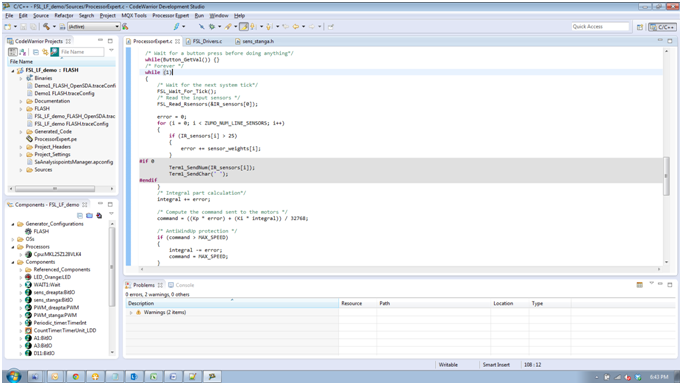
\includegraphics[width=1.0 \textwidth]{images/CodeWarriorMCU.png}}
  \vspace{-15pt}
  \caption{\label{fig:CodeWarrior-VedereDeAnsamblu} CodeWarrior for MCU - Vedere de ansamblu}
  \vspace{-20pt}
\end{figure}

\section{Compilarea proiectului}

\begin{wrapfigure}{r}{0.5\textwidth}
  \vspace{-20pt}
  \center{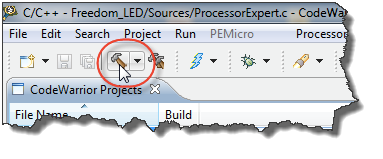
\includegraphics[width=0.5 \textwidth]{images/BuildProject.png}}
  \vspace{-15pt}
  \caption{\label{fig:CodeWarrior-CompilareProiect} Cum se poate compila proiectul}
  \vspace{-20pt}
\end{wrapfigure}

Pentru a compila proiectul, după ce în prealabil s-a generat codul folosind ProcessorExpert și voi v-ați scris codul vostru sursă, puteti folosi butonul din figura \ref{fig:CodeWarrior-CompilareProiect} sau de ce nu puteți folosi meniul principal și anume opțiunea \textit{Project $\rightarrow$ Build Project}. Indiferent de varianta aleasă rezultatul va fi același.

\begin{wrapfigure}{l}{0.5\textwidth}
  \vspace{-20pt}
  \center{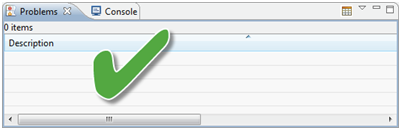
\includegraphics[width=0.5 \textwidth]{images/ProblemsView.png}}
  \vspace{-15pt}
  \caption{\label{fig:CodeWarrior-FereastraProblems} Când totul decurge bine...}
  \vspace{-20pt}
\end{wrapfigure}

Dacă totul a decurs cu bine, trebuie să nu avem erori în fereastra "Problems", așa cum evidențiază figura \ref{fig:CodeWarrior-FereastraProblems}.

\section{Descărcarea codului pe placă}

\begin{wrapfigure}{r}{0.5\textwidth}
  \vspace{-20pt}
  \center{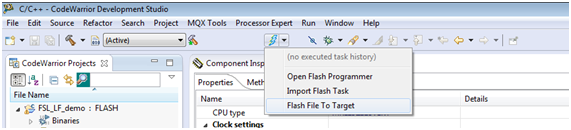
\includegraphics[width=0.5 \textwidth]{images/FlashProgrammer1.png}}
  \vspace{-15pt}
  \caption{\label{fig:CodeWarrior-FlashProgrammer1} Încărcarea codului pe placă}
  \vspace{-20pt}
\end{wrapfigure}

În urma compilării rezultă un executabil ce va trebui să fie flash-uit pe robot. Acest proces este realizat cu ajutorul unui instrument numit \textit{Flash Programmer}, iar figurile \ref{fig:CodeWarrior-FlashProgrammer1} și \ref{fig:CodeWarrior-FlashProgrammer2} vin să explice pașii ce trebuie urmăriți. Partea cea mai frumoasă o constituie faptul că aceste configurări vor fi făcute o singură dată. Ele sunt salvate local și pot fi refolosite de fiecare dată când este nevoie de ele.

\begin{wrapfigure}{r}{0.5\textwidth}
  \vspace{-20pt}
  \center{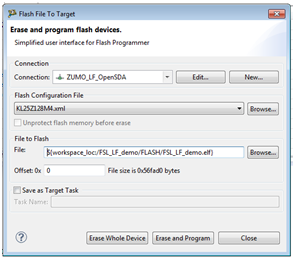
\includegraphics[width=0.5 \textwidth]{images/FlashProgrammer2.png}}
  \vspace{-15pt}
  \caption{\label{fig:CodeWarrior-FlashProgrammer2} Flash-uirea unui executabil}
  \vspace{-20pt}
\end{wrapfigure}

\section{Debugging}

\begin{wrapfigure}{l}{0.5\textwidth}
  \vspace{-20pt}
  \center{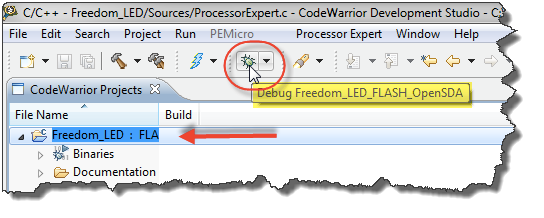
\includegraphics[width=0.5 \textwidth]{images/Debugging.png}}
  \vspace{-15pt}
  \caption{\label{fig:CodeWarrior-Debugging} Accesarea modului de debugging}
  \vspace{-20pt}
\end{wrapfigure}

Până să ajungeți la o versiune funcționalibilă, pe care să o puteți prezenta la concurs sau în cercul vostru de prieteni, va fi ceva de munca. Lucrurile vor fi abordate pas cu pas, va trebui de multe ori să faceți un debugging avansat pentru a înțelege ce e greșit în algoritmul vostru de robotul nu face ceea ce doriți voi să facă. În cazul în care vreți să puteți executa programul în modul debug (pas-cu-pas), puteți folosi butonul exemplificat în figura . Nu uitați, pentru a folosi acest mod, robotul trebuie să rămână conectat la laptop printr-un cablu. Ca alternativa - recomandată, de altfel – puteți folosi interfața serială pentru a trimite date dinspre robot spre laptop. Folsirea acestei interfețe seriale, vă va permite să faceți debugging folosind apeluri ale funcției "printf", cea mai primitivă metodă de a depana un program software. Din fericire, există și alte metode ceva mai avansate, cu rezultate mult mai bune, metode ce vor fi prezentate la ședințele tehnice.

\section{Processor Expert}

Processor Expert este un sistem de dezvoltare pus la dispozție de firma \textit{Freescale Semiconductor} ce poate regăsit deja instalat în \textit{odeWarrior for MCU}, prin intermediul căruia se pot crea și configura componente software ce generează cod sursă pentru microcontrollere produse de \textit{Freescale}. O astfel de componentă poate fi un driver, un algoritm sau o colecție de funcții software ce deservesc un obiectiv. O componentă poate fi, de exemplu, un driver ce permite accesul facil la pinii de intrare / ieșire puși la dispoziție de un microcontroller.

Folosirea Processor Expert înleșneste lucrul cu platforma hardware prin abstractizarea detaliilor de la nivelul low-level. Putem spune că avem de-a face cu o programare vizuală, în care este mai mult folosit mouse-ul decât tastatura. Noi, ca și programatori, vom avea mai multe de configurat setări și opțiuni pentru respectivul modul, pentru că mai apoi, codul să fie generat automat în funcție de inputul pe care l-am specificat. 

În cadrul acestui concurs, vom folosi Processor Expert. De ce? Răspunsul este foarte simplu. Cu ajutorul lui putem adăuga și configura componente, apoi genera cod sursă C pentru aceste componente. Codul generat va coexista cu codul C din proiectul nostru. Rezultatul acestei combinații de cod C scris manual și cel generat de \textit{Processor Expert} va fi compilat într-un singur executabil ce va fi folosit pentru construirea unui \textit{Line Follower}.

\subsection{Accesarea utilitarului}

\begin{wrapfigure}{l}{0.4\textwidth}
  \vspace{-20pt}
  \center{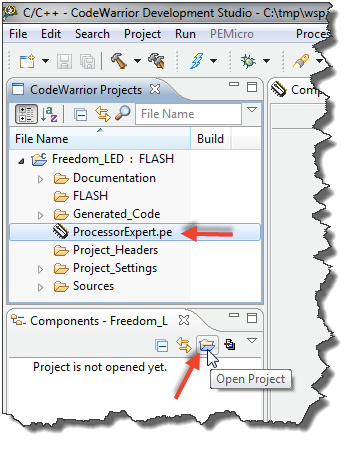
\includegraphics[width=0.4 \textwidth]{images/ProcessorExpert.png}}
  \vspace{-15pt}
  \caption{\label{fig:CodeWarrior-ProcessorExpert} Accesarea componentelor Processor Expert}
  \vspace{-20pt}
\end{wrapfigure}

După deschiderea proiectului în \textit{CodeWarrior for MCU}, în cazul în care fereastra \textit{Processor Expert} nu este vizibilă, va trebui să procedăm ca în figura \ref{fig:CodeWarrior-ProcessorExpert}.

\subsection{Adăugarea unui noi componente}

\begin{wrapfigure}{r}{0.3\textwidth}
  \vspace{-20pt}
  \center{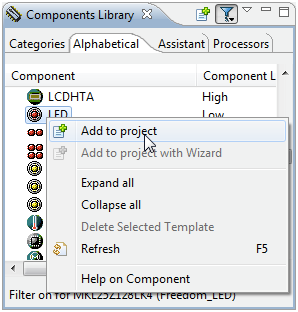
\includegraphics[width=0.3 \textwidth]{images/ProcessorExpertAdd.png}}
  \vspace{-15pt}
  \caption{\label{fig:CodeWarrior-ProcessorExpertAdd} Cum se adaugă o nouă componentă?}
  \vspace{-20pt}
\end{wrapfigure}

Înainte de a putea utiliza o componentă definită de acest utilitar, va trebui mai întâi, așa cum este și logic, să o adăugăm în cadrul proiectului nostru. Procesul de adăugare a unei componente este relativ simplu, fiind similar cu cel descris în figura \ref{fig:CodeWarrior-ProcessorExpertAdd}, din cadrul fereastrei de lucru \textit{Components Library}.

\subsection{Generarea de cod sursă}

După ce toate componentele necesare au fost adăugate și setate corect (sau după modificarea setaăilor unor componente) trebuie lansată o comandă prin care Processor Expert va fi înstiințat de faptul că trebuie să genereze codul sursă pentru componentele existente în proiect. Acest proces de înștiințare are loc doar prin apăsarea unui singur buton și anume - \textit{"Generate Processor Expert Code"}. După apăsarea butonului, utilitarul vă va rugă să aveți răbdare...

\begin{wrapfigure}{r}{0.3\textwidth}
  \vspace{-20pt}
  \center{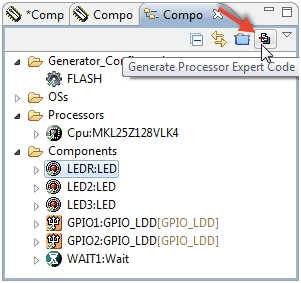
\includegraphics[width=0.3 \textwidth]{images/ProcessorExpertGenerate.png}}
  \vspace{-15pt}
  \caption{\label{fig:CodeWarrior-ProcessorExpertGenerate} Generarea de cod în Processor Expert}
  \vspace{-20pt}
\end{wrapfigure}

\textcolor{red}{Notă importantă:} Codul generat de Processor Expert conține zone ca cele de mai jos, rezervate special pentru codul pe care voi îl veți scrie. Nu încercați ăa modificați sau să scrieți cod în afara acestor zone, deoarece o noua generare a codului Processor Expert vă va șterge tot ce ați adăugat. Iar asta nu este foarte plăcut, pentru că va trebui să o luați de la capăt cu acele modificări manuale.

\lstinputlisting[caption=Inițializarea modulelor hardware, style=customc]{sources/generatingPExCode.lst}